%-------------------------------------------------------------------------
%\section{Kinematics of continua}

% *** EPS-Grafik ***
\begin{figure}[htb!]
\begin{center}
\footnotesize
%\includegraphics[height=5.973cm,width=11.507cm]{../figures/figure1.bmp}
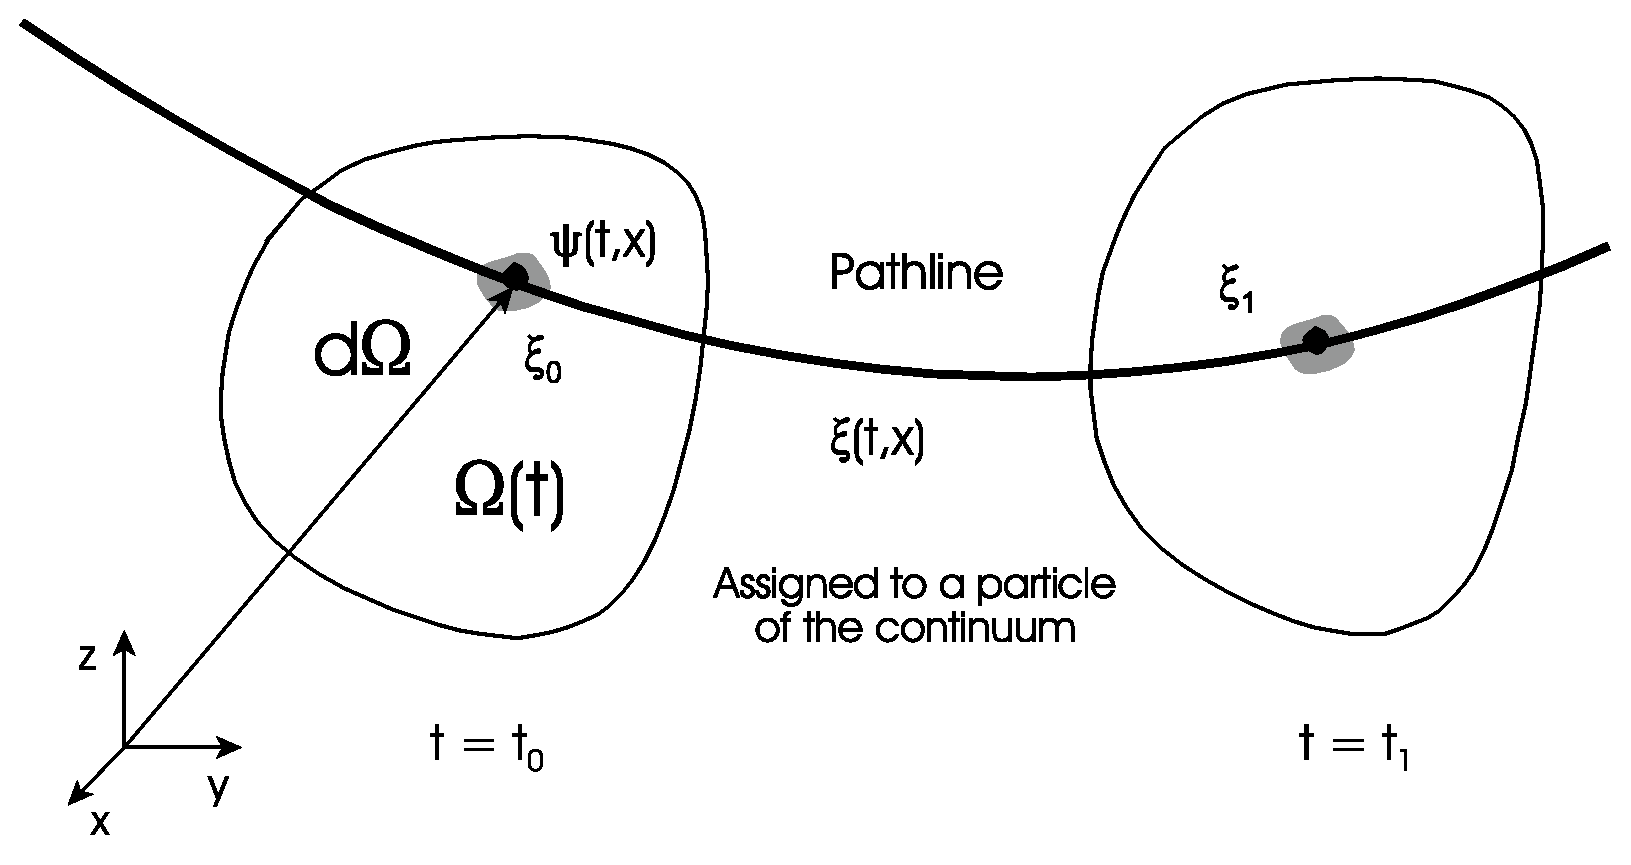
\includegraphics[width=0.8\columnwidth]{figures/mech1.eps}
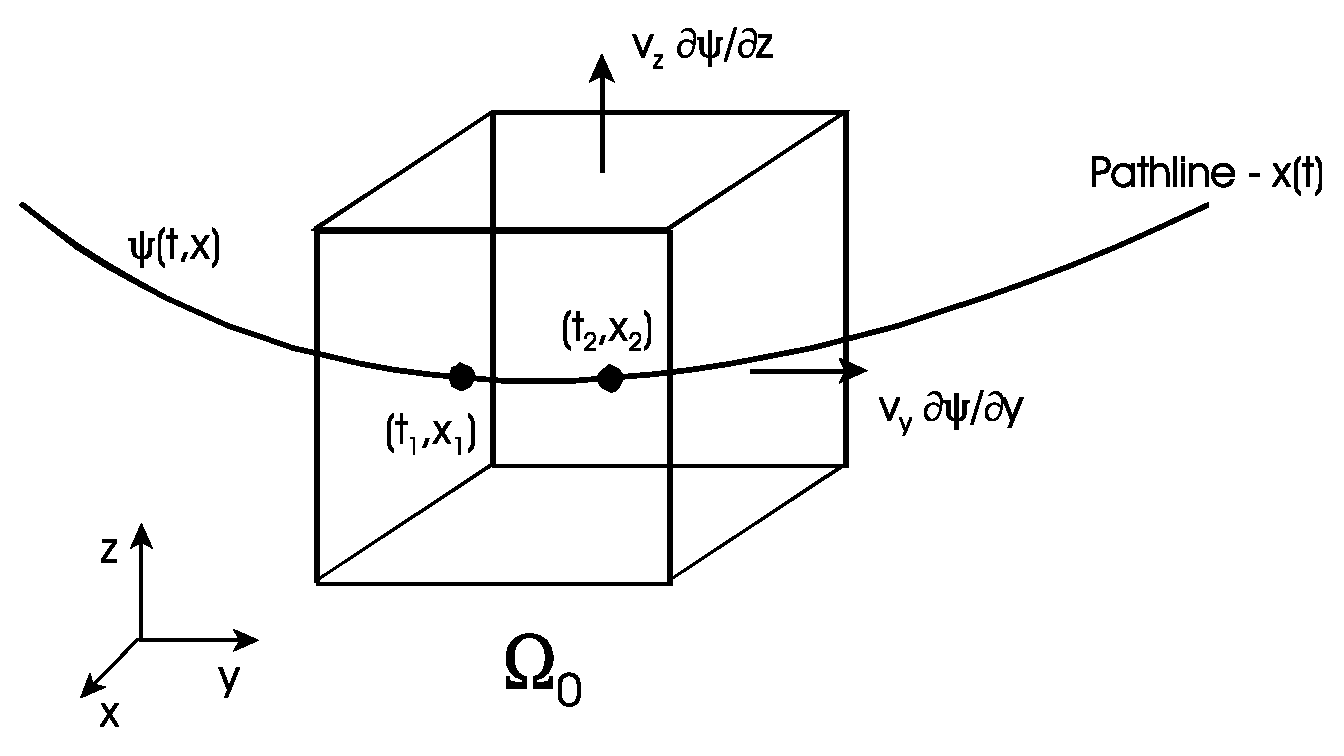
\includegraphics[width=0.8\columnwidth]{figures/mech2.eps}
\caption{Two basic descriptions of motion - Langrangian (top) and Eulerian principles (bottom), adopted from \cite{Kol:02}}
\label{fig:Euler-Langrange}
\end{center}
\end{figure}

\subsection{Lagrangian and Eulerian principles}
\label{sec:euler_lagrange}

In the {Lagrangian formulation}\index{formulation - Lagrangian} we
follow the quantity along a pathline, i.e. following particles
(Fig. \ref{fig:Euler-Langrange}, top). In the {Eulerian
formulation}\index{formulation - Eulerian} of motion we consider
variations of the quantity with respect to a fixed control
volume\index{volume - control} at fixed places (Fig.
\ref{fig:Euler-Langrange}, bottom).

A {pathline}\index{flow - pathline} is a curve along which a fixed
particle of a continuum moves during a sequence of time. Pathline
is Lagrangian concept of motion. A
{streamline}\index{flow - streamline} is a curve along which a
sequence of particles moves at a given time. By definition, the
tangent to a streamline coincides with the velocity vector at that
point. Streamline is Eulerian concept of motion. Note, for
unsteady flow the streamline may vary from one instant to the
next, whereas for steady flow streamlines remain unchanged with
time. For steady motion both pathlines and streamlines coincide.
Any particle will remain on a given streamline as time proceeds.
Additional terms associated with kinematics of continua are the
following (see also section \ref{sec:kinematics}).
